\documentclass[a4paper,11pt]{scrartcl}

%%% PAGE DIMENSIONS
\usepackage{geometry} % to change the page dimensions
\geometry{a4paper} 
\geometry{margin=85pt} % for example, change the margins to 2 inches all round

\usepackage{graphicx} % support the \includegraphics command and options

% \usepackage[parfill]{parskip} % Activate to begin paragraphs with an empty line rather than an indent

%%% PACKAGES
\usepackage{booktabs} % for much better looking tables
\newcommand{\tabitem}{~~\llap{\textbullet}~~}
\usepackage{array} % for better arrays (eg matrices) in maths
\usepackage{paralist} % very flexible & customisable lists (eg. enumerate/itemize, etc.)
\usepackage{verbatim} % adds environment for commenting out blocks of text & for better verbatim
\usepackage{subfig} % make it possible to include more than one captioned figure/table in a single float
\usepackage{multirow}
\usepackage{hyperref}
\usepackage{xcolor}
\hypersetup{
    colorlinks,
    linkcolor={red!50!black},
    citecolor={blue!50!black},
    urlcolor={blue!80!black}
}

% code listing
\usepackage{minted}
\usemintedstyle{autumn}
\def \scriptPath{D:/Studie/Master/ExperimentationProject/Scripts}
\def \flashWrapPath{D:/Studie/Master/ExperimentationProject/SourceProjects/NameResolution/src}

\usepackage{caption}

\usepackage{cite}

%%% HEADERS & FOOTERS
% \usepackage{fancyhdr} % This should be set AFTER setting up the page geometry
% \pagestyle{fancy} % options: empty , plain , fancy
% \renewcommand{\headrulewidth}{0pt} % customise the layout...
% \lhead{}\chead{}\rhead{}
% \lfoot{}\cfoot{\thepage}\rfoot{}

%%% SECTION TITLE APPEARANCE
\usepackage{sectsty}
\allsectionsfont{\sffamily\mdseries\upshape} % (See the fntguide.pdf for font help)
% (This matches ConTeXt defaults)

%%% ToC (table of contents) APPEARANCE
\usepackage[nottoc,notlof,notlot]{tocbibind} % Put the bibliography in the ToC
\usepackage[titles,subfigure]{tocloft} % Alter the style of the Table of Contents
\renewcommand{\cftsecfont}{\rmfamily\mdseries\upshape}
\renewcommand{\cftsecpagefont}{\rmfamily\mdseries\upshape} % No bold!

%% Document Header
\title{Assessing Bytecode Optimizations for the Adobe Flash Player}
\subtitle{Experimenting With Method Dispatch in a (Semi-) Black Box}
\author{Sije Harkema - 3631230}

\begin{document}
\maketitle

\section{Introduction}
\label{sec:introduction}

This research was conducted as part of an experimentation project at Utrecht University\footnote{For completeness sake, conducted as part of INFOMEPCS1 for partial completion of the Computer Science master degree.}. In 2011, Middelkoop \textit{et. al.} \cite{Middelkoop2011} performed a study on instrumentation of ActionScript (AS) programs through the means of bytecode manipulation. As part of this project the authors gained some rudimentary knowledge on how method dispatch should work in the ActionScript Virtual Machine (AVM). In an informal setting it has been hinted that method dispatch can be a great candidate for optimization of Flash programs. This is further confirmed by a notice in the very bottom of the specification document for the AVM \cite{Adobe2007}, which briefly states how sometimes \texttt{callproperty}, \texttt{callproplex} and \texttt{callpropvoid} can be replaced by \texttt{callmethod} and \texttt{callstatic}, which skip an intermediate lookup step for the property name. A more thorough explanation will be presented later in this report.

This experimentation project was setup to explore what is possible with this kind of optimizations. It should give an estimation of how hard is to achieve, possibly in an automated way, and how much impact these optimizations have. At section \ref{sec:ecosystem} we will look into the Flash ecosystem to see how the development cycle is typically done and how the ActionScript language, the ActionScript Virtual Machine and the Adobe Flash Player relate to each other. Section \ref{sec:methodology} shows how we setup and execute the different experiments, with the results and basic analysis in section \ref{sec:results}. We conclude in section \ref{sec:discussion} with what the implications are of the results.

Why are we conducting this research? The Flash ecosystem provides a way of developing ``high-impact, rich Web content'' \cite{AdobeSystems}, but is also used in a standalone setting. Despite being highly critized for the numerous security vulnerabilities \cite{Van-Acker2012, Symantec2016}, and major platforms and browsers moving away (due the large attack surface \cite{LaForge2016, Seitz2009}), it is still widely employed in millions of devices \cite{AdobeSystemsa}.

\section{Flash ecosystem}
\label{sec:ecosystem}
The \textit{Adobe Flash Player} is the main\footnote{Alternatives exists, some copying the purpose of the Adobe Flash player, others have a different purpose.  On Linux, Gnu Gnash is popular. The Unity Web player has some support for interop for it, and Lightspark is an actively developed player and browser plugin. } runtime for \texttt{.swf} files. In short, it is a container format for ActionScript Bytecode, and optionally multimedia files. The main component is an implementation for the \textit{ActionScript Virtual Machine (AVM)}. The Flash player is mainly used as a browser plugin, though standalone variants also exist\footnote{This has been superseded by the \textit{Adobe Air} runtime system, where a slim runtime is distributed with every application.}. As plugin, it is limited by a number of security precautions, like interactions with the local filesystem and performing network requests to other domains. For interaction with the embedding web page there is some basic functionality (like calling defined javascript functions).

The \texttt{.swf} files are generated by a variety of products. Some focus on animation (Adobe Animate, Adobe LiveMotion, Adobe Illustrator)\footnote{Also: ToonBoom, Apple Keynote, and dozens others.}, some on the scripting side (Adobe Flash Builder, FlashDevelop, Haxe)\footnote{Also: SWFTools, Ming library, CrossBridge and dozens others.}. Scripting is generally achieved by ActionScript. For the execution of the ActionScript code, Adobe constructed a Virtual Machine specification. The second generation of this specification, the AVM2, is the one we will focus on. This was designed to work with ActionScript 3.0.

Before we will dive into the parts of AVM2 that are relevant, we shortly discuss compilation and decompilation. Like some major compiled languages (note, for AS it is compilation to virtual machine bytecode, not native machine code) there is a `dumb' compiler, in this case \texttt{ASC (asc.jar)}, and a wrapper, \texttt{mxmlc}, which understands \textit{mxml} in which more complicated compilation configurations can be specified\footnote{And one can specify UI layouts in it.}. The relation between these two has not been clearly stated as far as the author knows, though it has been stated by \cite{smith2009} the former is ``less flexible'' but ``might be faster for special purposes''. Additionally, preliminary research shows \texttt{ASC} \textit{might} produce different and more verbose code, of which an example will be discussed in section \ref{sec:results}. The compilers are packaged together with an \textit{SDK}. A commonly used \textit{SDK} is \textit{Apache Flex}, until 2012 known as \textit{Adobe Flex}. For decompilation several third-party tools are available. We use both \textit{JPEX Free Flash Decompiler v.9.0.0} (with GUI) and RABCDAsm (with CLI).

\subsection{AVM2}
Anything targetting the AVM2 can utilize a number of specific instructions. For every instruction is specified: the opcode, any arguments to the opcode, how the stack is manipulated and a description. The description will also specify any other effects like loading of the local registers or the semantics of exceptions. To illustrate the primary subject of this project, we use the code from listing \ref{lst:basic}.

\begin{listing}
\begin{minted}
[
frame=leftline,
framesep=2mm,
baselinestretch=1.2,
%bgcolor=LightGray,
fontsize=\footnotesize,
linenos
]{actionscript}
package 
{
	public class C
	{
		public function f():void 
		{
			
		}
	}

	public class Main 
	{
        	public function Main()
		{
			var _C:C = new C;
			_C.f();
		}
	}
}
\end{minted}
\caption{Basic call}
\label{lst:basic}
\end{listing}

This shows a very basic program: no overrides, no class hiërarchy and a single method\footnote{There is a distinction between `method' and `function',  which follows the usual convention. Methods are functions defined as part of a class definition, or when dynamically attached to a class instance.} Decompilation will give us for the call instruction (line 16): \\
\texttt{callpropvoid Qname(PackageNamespace(""),"f") 0} \\
The description of \texttt{callpropvoid} describes how the \textit{multiname} (namespacing not of importance here) is an index into the multiname constant pool, and continues: ``The property specified by the multiname ... is resolved on the object'' \cite{Adobe2007}. Property means a specific trait kind here. Traits are a specific AVM2 concept, and can represent for example\footnote{Also class initializers (not the same as instance initializers), functions and `slots' (similar to constants).} getters, setters, constants and methods. Upon instance construction, each instance gets a traits table. Each method trait has an integer \texttt{disp\_id} (of which next to nothing is known) and an \texttt{index }that points into the \texttt{method} array of the \texttt{abcFile}.

The \texttt{.swf} container permits embedding multiple \texttt{abcFile} structures. The AVM2 specification has more information on this construct. For all our purposes, we limit ourselves to a single \texttt{afcFile}. This will have no problematic consequences, as the runtime operates as far as we are concerned on a single structure. \\
The \texttt{method} array mentioned holds the actual method execution information\footnote{Technically the method signatures and method bodies are split up, because of native methods which have no body.}. It is a global array.

There is another method invocation opcode: \texttt{callmethod}. This receives as first argument an integer named \texttt{index}, described as ``the index of the method to invoke on receiver''. Receiver should be an object on the stack at a depth dependent on the argument count. A later fragment in the opcode description shows: ``The method at position \textit{index} on the object \textit{receiver} is invoked with ....''. Preliminary research showed this index is also referred to (in error messages for example) as \texttt{disp\_id}. The AVM2 specification has an interesting section on optimizing method dispatch by using \texttt{callmethod} instead of \texttt{callproperty} (or similar opcodes). It refers to a non-existent \texttt{trait\_method} structure on the \texttt{abcFile}, and additionally to a ``method table''. (This ``method table'' is said to have non-zero offsets.) The experiments will clear up some of this confusion. The main purpose of the compiler hint subsection was to state that it is possible to provide some index to \texttt{callmethod} to avoid a name lookup.


\section{Methodology}
\label{sec:methodology}

The goal is to test how much performance we can gain by changing \texttt{callproperty} opcodes with \texttt{callmethod} (not blindly of course, taking into account stack issues etc.). The Flash player however will reject any program containing any \texttt{callmethod} instruction. The runtime has a verification mechanism built-in, which works in different stages of the execution. This situation will trigger a fatal error\footnote{There are two different error messages. ``VerifyError: Error 1072: Disp\_id 0 is illegal.'' or ``VerifyError: Error 1051: Illegal early binding access to \textit{classname}.'' } immediately.

So far we considered the runtime to be a completely black box. Adobe however hosts a project on GitHub called \textit{avmplus}. The documentation is sparse, development is done in private and the workings are quite difficult to comprehend due to its size\footnote{\textit{sloccount} shows 491.929 lines of code in total}. Also, its place in the current Flash player/plugin is not specified. We can however see why our \texttt{callmethod} will probably always fail: \textit{core/verifier.cpp} line 1838 has the error hardcoded in. A comment explains the reason: problems will arise when the class \texttt{Object} has methods.

To still come to answers for our project, we use 2 approaches. We can infer some behaviour about method dispatch and lookup times for names by building a case with a large number of classes and methods, test it and then change how many times we call a certain method. Any kind of non-constant lookup will show. We will refer to this experiment as the ``reorder experiment'',  and work this out in section \ref{sec:methodology-reorder}. \\
We also changed and compiled \textit{avmplus} to silence the error in the hopes of still having a well executing program. This is discussed in \ref{sec:methodology-callmethod}. 

\subsection{Common operations, common testcase}
\label{sec:methodology-common}
Both experiments require a useful testcase. The testcase should represent the situation which would benefit the most from optimizations. Despite earlier mentioning of the \textit{avmplus} code, we still have to approach the runtime as a black box. Considering the structures involved in method dispatch, we choose our testcase to have a large number of classes with a large number of methods, and will have the method bodies to be extremely trivial. We also generate a number of subclasses, as the AVM2 specification hints briefly (section 4.8.5) it might affect dispatch, where only the even methods are overridden. Listing \ref{lst:classes} shows how the outline of such classes would look. For the calling code, we want a high amount of calls to all methods. The calling code length should not exceed impractical limits though\footnote{For debug, edit is permitted to be slow, but doable within an hour.}, so loops address that. (Listing \ref{lst:naive} shows the naive way.) Some JIT-mechanism\footnote{Just In Time optimizations for hot paths} might optimize with repeated calling. We use loops, then break up the loops in \textit{n} \textit{sub}-loops, then randomize the order of them all. This is demonstrated in listing \ref{lst:blocks} (in reality the loop limits would exceed 1 of course).

We wrote a set of common files that aid in generating these AS classes, methods and calling code. This code works by having some basic templates where some missing information gets substituted in.

\begin{minted}
[
frame=leftline,
framesep=2mm,
baselinestretch=1.2,
%bgcolor=LightGray,
fontsize=\footnotesize,
linenos
]
{actionscript}
public class C1
	{
		public function work1():String
		{
			var k:String = 'C1' + 's1';
			return k;
		}
		
		...
		
		public function work50():String
		{
			var k:String = 'C1' + 's50';
			return k;
		}
	}
	
public class C11 extends C1
	{
		
		override public function work2():String
		{
			var k:String = 'C11' + 's2';
			return k;
		}
		
		override public function work4():String
		{
			var k:String = 'C11' + 's4';
			return k;
		}
		
		...
		
		override public function work50():String
		{
			var k:String = 'C11' + 's8';
			return k;
		}
	
	}
\end{minted}
\captionof{listing}{Testcase class declarations \label{lst:classes}}

\begin{minted}
[
frame=leftline,
framesep=2mm,
baselinestretch=1.2,
%bgcolor=LightGray,
fontsize=\footnotesize
]{text}
Impractical:
work1()
work1()
work1()
work2()
work2()
work2()
...
work50()
work50()
work50()

Ordered loops:
for i in 1..3:
    work1()
for i in 1..3:
    work2()
...
for i in 1..3:
    work50()
\end{minted}
\captionof{listing}{Naive calling \label{lst:naive}}

\begin{minted}[
frame=leftline,
framesep=2mm,
baselinestretch=1.2,
%bgcolor=LightGray,
fontsize=\footnotesize
]{text}
for i in 1..1:
    work50()
for i in 1..1:
    work1()
for i in 1..1:
    work50()
for i in 1..1:
    work2()
for i in 1..1:
    work2()
for i in 1..1:
    work1()
for i in 1..1:
    work50()
for i in 1..1:
    work2()
for i in 1..1:
    work2()
for i in 1..1:
    work1()
\end{minted}
\captionof{listing}{Blocked randomized loops\label{lst:blocks}}

\subsection{Reorder experiment}
\label{sec:methodology-reorder}
In this particular experiment a key assumption is we have no way of using \texttt{callmethod} to skip the name lookup, but the lookup itself might be prone to optimizations. In a linear search strategy it would be possible to reorder the lookup table to have the most commonly used methods in front. Determining what these most commonly used methods is out of scope for this research.

Our testcase will have $p$ classes, each of which has $q$ subclasses. Every class has  $n$ methods. Additionally, in the calling code, we split the loops in $r$ blocks, and $s$ is the amount of total calls for a class, such that in the equally distributed case every method is called $ s / n $ times, and the upper loop limit for each block is $ (s / n) / r $. 

When `optimizing' we set the new limits on all blocks such that the one \textit{target} method of each class is called $ 0.9 * s$, and every other method is called $ 0.1 * s / (n-1) $. The hypothetical linear search strategy would be impacted by this. (While this is done on the bytecode level in the implementation it could coincidentally also have been achieved on the source level for this particular case.)

The test pipeline is architectured to automatically run a series of steps on all source projects it can find (in a given start directory). It will compile the project with $n$ different compilers\footnote{Options are:  Adobe Flex Compiler (mxmlc) 3.2.0 build 3958, Apache Flex Compiler (mxmlc) 4.9.1 build 1447119, 
Apache Flex Compiler (mxmlc) 4.15.0 build 20160104 and Adobe ActionScript Compiler (mxmlc) Version 2.0.0 build 354194}. Compilers theoretically could execute optimizations themselves in the production of bytecode, and different generations and variants are therefore included. It will check whether a routine for optimization is included in the script for the project and apply it, otherwise an identity transformation (copy) is performed. The runtime can behave differently in significant ways. The pipeline therefore executes the $2n$ \texttt{.swf} files in a range of different runtimes which encompass the standalone player and the plugin on different operating systems\footnote{On Windows the following: flashplayer\_23\_sa, flashplayer9r280\_win\_sa and plugin version (24,0,0,186) in FireFox 50.1.0.}.  For results not to be  influenced by other factors, the pipeline is carefully constructed to be fully automatic while isolating runs and detecting failures.

The main code is included in listing \ref{lst:reorder-run-main}. The source for all code, including preliminary assertions, templates and helpers can be found in appendix \ref{sec:resources}.

\inputminted[
frame=leftline,
framesep=2mm,
baselinestretch=1.2,
%bgcolor=LightGray,
fontsize=\footnotesize,
linenos,
firstline=285,
lastline=327
]
{python}{\scriptPath/run_reorder_exp.py}
\captionof{listing}{run\_reorder\_exp.py: main function \label{lst:reorder-run-main}}

All the projects are supplied with some ActionScript wrapping code to do the profiling. When executing, this wrapping code will execute the testcase a fixed amount of iterations. Each iteration is timed, and the results are indirectly written to a log file, accompanied by the environment it was executed in. Because of security restrictions, the results are sent through a simple http server which logs to a database. For tests on other platforms the script will additionally store all created executables online.

\subsection{Callmethod experiment}
\label{sec:methodology-callmethod}
As has been discussed, there is a possibility to utilize the \textit{avmplus} code in an experiment. This can be manually compiled under certain conditions. This process is described in appendix \ref{sec:buildavmplus}. This experiment follows the original approach for optimizing method dispatch. A testcase would be compiled, some mechanism would alter the bytecode to replace call opcodes to use \texttt{callmethod}. The compilation of \textit{avmplus} results in a binary named \textit{avmshell}. Making this binary execute code compiled with the \textit{mxml} compilers is not practical\footnote{It will error on a lack of builtin types, which the normal player has included by itself, but for \textit{avmshell} needs to be included explicitly. This uses the file \textit{builtins.abc}.}. The experiment is split into two stages. Stage 1 generates a testcase identical to the "reorder experiment", with the exception that all code is in a single file, mostly for convenience\footnote{When invoking \textit{avmshell} one would otherwise have to include all files separately, which for a small amount is annoying, and for a large amount is impossible because of shell limitations.}. 

Stage 2 will compile the testcase using \texttt{ASC (asc.jar)} with optimizations enabled and disabled. The bytecode is copied, and all lines matching ``\texttt{callproperty ... work(i)}'' are replaced with ``\texttt{callmethod i 0}''. Both versions get executed a fixed amount of iterations, and for each iteration resource usage (cpu time and memory usage) gets logged. We also test the effects of the runtime flag which forces JIT. The \texttt{main} function of stage 2 is included in listing \ref{lst:callmethod-run2-main}.

\inputminted[
frame=leftline,
framesep=2mm,
baselinestretch=1.2,
%bgcolor=LightGray,
fontsize=\footnotesize,
linenos,
firstline=167,
lastline=191
]
{python}{\scriptPath/run_callmethod_exp_stage2.py}
\captionof{listing}{run\_callmethod\_exp\_stage2.py: main function \label{lst:callmethod-run2-main}}


\section{Results}
\label{sec:results}

\subsection{Reorder experiment}
\label{sec:results-reorder}

We present in table \ref{tbl:reorder-results} the results for the reordering experiment, where the optimization step is changing the distribution of the calls, some \textit{target} method gets 90\% of the calls. The testcase is configured to have 8 base classes, each of which has 8 subclasses. There are 50 methods defined for the classes\footnote{The subclasses override only the even methods, but inherit the rest} , and the number of calls per class is 400.000.  The loops have been divided up in 4 blocks. The calling code will thus have total of 14.400 loops, and a total of 28.800.000 method calls will be made. 

\begin{table}[h!]
\footnotesize
\begin{center}
 \begin{tabular}{|c|c|c|c|c|c|c||c|c|c|c|c|c|} 
 \hline
 \multicolumn{4}{|c|}{ } & \multicolumn{3}{|c||}{ work1 } & \multicolumn{3}{|c|}{ work25 } & \multicolumn{3}{c|}{work50}\\
 \hline
compiler & version & standalone & optimized & avg & std & n & avg & std & n & avg & std & n \\
\hline
0 & 0 & 1 & 0 & 2137.12 & 69.27 & 17 & 2137.12 & 69.27 & 17 & 2137.12 & 69.27 & 17 \\ 
0 & 0 & 1 & 1 & 745.87 & 40.61 & 15 & 719.92 & 5.28 & 13 & 731.67 & 9.07 & 15 \\ 
0 & 1 & 1 & 0 & 3304.58 & 72.10 & 19 & 3304.58 & 72.10 & 19 & 3304.58 & 72.10 & 19 \\ 
0 & 1 & 1 & 1 & 1111.94 & 41.80 & 16 & 1084.80 & 9.67 & 15 & 1083.56 & 14.65 & 16 \\ 
0 & 2 & 0 & 0 & - & - & - & - & - & - & - & - & - \\ 
0 & 2 & 0 & 1 & - & - & - & - & - & - & - & - & - \\ 
0 & 3 & 0 & 0 & 3156.33 & 47.04 & 12 & 3156.33 & 47.04 & 12 & 3156.33 & 47.04 & 12 \\ 
0 & 3 & 0 & 1 & 1072.64 & 5.46 & 39 & 1079.92 & 6.84 & 39 & 1097.05 & 15.30 & 38 \\ 
3 & 0 & 1 & 0 & - & - & - & - & - & - & - & - & - \\ 
3 & 0 & 1 & 1 & - & - & - & - & - & - & - & - & - \\ 
3 & 1 & 1 & 0 & 142.92 & 15.99 & 13 & 142.92 & 15.99 & 13 & 142.92 & 15.99 & 13 \\ 
3 & 1 & 1 & 1 & 63.40 & 20.02 & 10 & 76.14 & 7.62 & 14 & 77.50 & 18.34 & 14 \\ 
3 & 2 & 0 & 0 & 190.32 & 18.68 & 19 & 190.32 & 18.68 & 19 & 190.32 & 18.68 & 19 \\ 
3 & 2 & 0 & 1 & 92.16 & 8.64 & 19 & 89.63 & 11.68 & 19 & 80.63 & 16.25 & 19 \\ 
3 & 3 & 0 & 0 & 135.68 & 4.82 & 19 & 135.68 & 4.82 & 19 & 135.68 & 4.82 & 19 \\ 
3 & 3 & 0 & 1 & 48.21 & 0.54 & 19 & 49.37 & 1.67 & 19 & 53.84 & 8.77 & 19 \\ 
\hline
\end{tabular}
\end{center}
\caption{Reorder results ; seed set to $42^3$ }
\label{tbl:reorder-results}
\end{table}

\begin{table}[h!]
\begin{center}
\begin{tabular}{c|c}
0 & Adobe Flex Compiler (mxmlc) 3.2.0 build 3958 \\
3 & Adobe ActionScript Compiler (mxmlc) Version 2.0.0 build 354194 \\
\end{tabular}
\end{center}
\caption{Legend for the compilers used}
\label{tbl:reorder-compilers}
\end{table}

\begin{table}[h!]
\begin{center}
\begin{tabular}{c|c}
0 & WIN 9,0,280,0 \\
1 & WIN 23,0,0,185 \\
2 & WIN 24,0,0,186 \\
3 & MAC 24,0,0,186 \\
\end{tabular}
\end{center}
\caption{Legend for the runtimes used}
\label{tbl:reorder-runtimes}
\end{table}

A number of combinations for the compiled files and runtimes is incompatible, and will silently fail (indicated with a dash). For this experiment we used only the oldest and newest compiler\footnote{The times for the files compiled with the other compilers were between the presented results.}. Compiler 0 (oldest) generates severely worse code it seems. Upon inspection, the difference is in the construction of the classes upon which the methods are called\footnote{The old compiler will first push a \texttt{null} value on the stack for every class, then coerce it to the required type. It will then also call the constructor for the class  with \texttt{constructprop}, which will override the coerced value. The newer compiler will only do the second part.}. This indicates the construction of the classes overshadows the execution of methods, which contradicts other preliminary tests scaling the experiment to different sizes. No explanation for this could be constructed\footnote{An error in the manual comparison of the decompiled files is the most likely cause, so it is assumed the construction does not play too much of a role}.

\begin{figure}[h!]
\centering
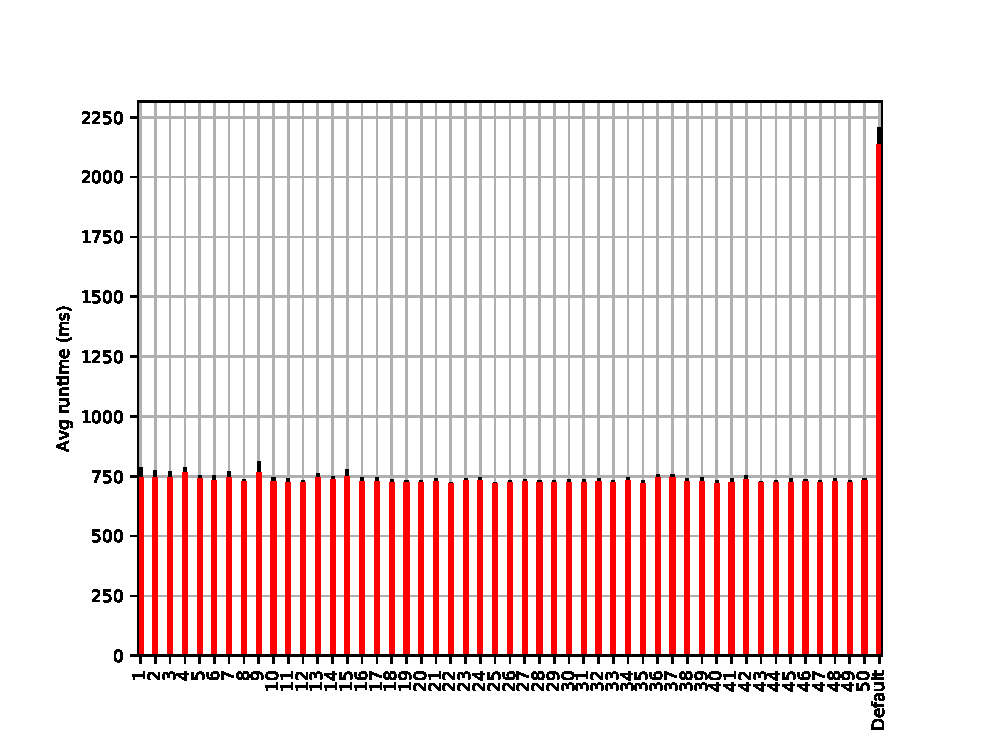
\includegraphics[scale=1.1]{D:/Studie/Master/ExperimentationProject/Results/reorder_comp0_version0.eps}
\caption{Runtimes per target, compiler=0, version=0}
\label{fig:reorder-plot}
\end{figure}

It has to be noted that in every run the first iteration for the benchmarking was an extreme outlier, despite the fact that the benchmarking really only runs the benchmark and not the wrapping code for the result logging. We excluded these outliers. Because of some practical issues \footnote{The network was an issue for communication from OSX with the logging server, when running the compiler=0 executables on OSX the stop criteria was never set correctly, the log utility was sometimes buggy, etc...} the amount of iterations varies. 

For every target, the runtime of the optimized version drops substantially to less than 50\% of the non-optimized version. The difference between targets is not clear from table \ref{tbl:reorder-runtimes} alone. The plot in figure \ref{fig:reorder-plot} shows for all targets the runtime for the configuration compiler=0, version=0. (Other plots are included in appendix \ref{sec:additional-data}.) Caching on some level (cpu, player or elsewhere) is the probable cause for the lower runtimes of the optimized applications.

Regarding player versions: the old player and compiler make a better match than the old compiler with newer players, but overall there does not seem to be a clear pattern. (It has been rumored the OSX Flash player is severly (5-10x) slower than other platforms, which is not the case here. The player tested was bundled with Google Chrome.) 

Everything has been duplicated with another seed to account for the influence of the order of the calls. The data for where the seed is set to $42^2$ can also be found in section \ref{sec:additional-data}. It has been omitted here because it shows almost identical results.


\subsection{Callmethod experiment}
\label{sec:results-callmethod}

The testcase for this experiment is configured identically to the testcase for the reorder experiment. The whole program is ran 10 times. The resource usage has been monitored, both cpu time in user mode and system mode. The memory recordings have been omitted because they do not change\footnote{These can be retrieved from the data sources specified in appendix \ref{sec:resources}.}. Table \ref{tbl:callmethod-results} shows both the user mode and system mode times, in milliseconds.

\begin{table}[h!]
\begin{center}
\begin{tabular}{c|c|c|c|c|c|c|c|c|}
seed & compile\_flags & run\_flags & optimized & avg\_utime & std\_utime & avg\_stime & std\_stime & n \\
\hline
1764 & -optimize & -Djitordie & 0 & 6875.2 & 528 & 109.0 & 29 & 10 \\
1764 & -optimize & -Djitordie & 1 & 6900.5 & 383 & 102.0 & 20 & 10 \\
1764 & -optimize &  & 0 & 4799.8 & 62 & 49.9 & 17 & 10 \\
1764 & -optimize &  & 1 & 4844.6 & 89 & 37.2 & 10 & 10 \\
1764 &  & -Djitordie & 0 & 6766.6 & 379 & 103.0 & 18 & 10 \\
1764 &  & -Djitordie & 1 & 6801.9 & 411 & 106.1 & 24 & 10 \\
1764 &  &  & 0 & 4901.2 & 69 & 49.0 & 12 & 10 \\
1764 &  &  & 1 & 4909.1 & 71 & 41.7 & 14 & 10 \\
74088 & -optimize & -Djitordie & 0 & 7122.3 & 384 & 147.2 & 53 & 10 \\
74088 & -optimize & -Djitordie & 1 & 6680.7 & 176 & 111.3 & 22 & 10 \\
74088 & -optimize &  & 0 & 4797.9 & 23 & 37.0 & 14 & 10 \\
74088 & -optimize &  & 1 & 4802.5 & 53 & 43.0 & 12 & 10 \\
74088 &  & -Djitordie & 0 & 6700.7 & 220 & 110.7 & 19 & 10 \\
74088 &  & -Djitordie & 1 & 6793.5 & 192 & 103.3 & 18 & 10 \\
74088 &  &  & 0 & 4863.7 & 72 & 44.8 & 9 & 10 \\
74088 &  &  & 1 & 4860.3 & 81 & 42.8 & 12 & 10 \\

\end{tabular}
\end{center}
\caption{Callmethod results}
\label{tbl:callmethod-results}
\end{table}

We first see the runtime is notably affected by the different compilation and runtime configurations. The variation in performance is minimal, with standard deviation never exceeding 10\% of the mean, where the runs with JIT forced vary the most, these are also the slowest by a great margin. The optimized version was slower in 6 out of 8 cases, where the differences range from $-1.4$\% to $0.1$\% (with one outlier of $6.2$\%). Although upon glance it seems there is no difference, a Wilcoxon Rank Sum Test was performed\footnote{A z-value of $-0.10502$ was found. To confirm the Wilcoxon test, a Two-Sample t-Test was performed. The test agreed.} indicating no significant difference between optimized and non-optimized was found.

Some testing was done to incorporate the idea of the reorder experiment in this experiment. When all \texttt{callmethod} instructions call to a single method (so 100\% of calls to a target method), the runtime is identical to what was shown in table \ref{tbl:callmethod-results}.

\newpage

\section{Conclusion \& Discussion}
\label{sec:discussion}

The goal of this project was to gain insight in how rewarding optimizations regarding method dispatch could be. Because the Adobe Flash player is a black box, we conducted an experiment that could expose some information regarding the internal layout of methods. The reorder experiment shows it is improbable such optimizations would have significant effect. It is likely there is no simple linear search strategy applied for method lookup internally, though other internal optimizations might have affected this conclusion.

With the callmethod experiment we tested the proposed optimization directly. It was however shown the runtime characteristics of \textit{avmshell} are very different from the common players, which hinders comparison. Regardless of that there was shown no improvement of runtime with the direct use of the \texttt{callmethod} instruction. This study did not include research into the \textit{avmplus} source code, but brief browsing through it has shown some hashing mechanisms working with \textit{multinames}\footnote{In the various \textit{core/MultinameHashtable*} files for example.}, which supports the other results.

All results imply the optimizations would not have the desired effects. However, there are some open questions left. The explanation for the large performance gap between files from the old and the new compiler was not satisfactory, and could change how good the testcase really is. The internal hashing mechanism which \textit{avmplus} seems to use might alter the performance when the testcase triggers a lot of collisions for example. The framework developed for this research lends itself for other optimization routines as well, and even trivial optimizations like unnecessary coercions are still not obsoleted by current-day compilers.

\section{Acknowledgements}
I would like to thank Jurriaan Hage for the ideas, feedback and patience, William Maddox for the \textit{avmplus} help, and Webeau for their flexibility in dealing with my work hours.


\newpage

\section{Bibliography}
\bibliographystyle{plain}
\bibliography{D:/Studie/Master/ExperimentationProject/Report/refs}

\appendix

\section{Resource repository}
\label{sec:resources}

A git repository is hosted at \url{https://gitlab.com/harkemasije/flash-experimentation-project/tree/master} (mirrored at \url{https://github.com/afraca/flash-experimentation-project}). It has the code that generates all intermediate results. It has a \textit{sqlite} datbase file with all the raw results. It also has the ActionScript wrapping code for the benchmarking. Additionally it has all calculated results that were not included here.


\section{Build instructions \textit{avmplus}}
\label{sec:buildavmplus}

Instructions for Linux. Use Python 2 for this (2.7.12 was tested as working). (Note there is an older incomplete identically named repository under the organization \textit{adobe-flash}.)

\begin{itemize}
\item \begin{verbatim} git clone https://github.com/adobe/avmplus.git \end{verbatim} 
\item \begin{verbatim} cd avmplus \end{verbatim}
\item \begin{verbatim} mkdir bin-release && cd bin-release \end{verbatim}
\item \begin{verbatim} python ../configure.py \end{verbatim}
\item Install \texttt{default-jre} 
\item Download redtamarin sdk, navigate to it's lib directory, place that \texttt{asc.jar} in \textit{avmplus/utils} (Do not use \texttt{asc2.jar})
\item Remove from \textit{avmplus/bin-release/Makefile} the \texttt{-Werror} and add \texttt{-Wno-narrowing -fpermissive} to c++ options
\item Execute \texttt{make}
\end{itemize}

There is now an executable avmshell in \textit{avmplus/bin-release/shell}

\section{Additional data}
\label{sec:additional-data}

(Easy to browse results can be found at appendix \ref{sec:resources})

Reorder experiment results, layed out like table \ref{tbl:reorder-results}. Seed is $42^2$. Runs for OSX were not performed. 
\begin{verbatim}
compiler;version;standalone;optimized;avg;std;n;avg;std;n;avg;std;n
0;0;1;0;2083.95;39.92;19;2083.95;39.92;19;2083.95;39.92;19
0;0;1;1;726.12;19.81;16;740.17;23.21;18;742.20;22.95;15
0;1;1;0;3095.00;74.53;18;3095.00;74.53;18;3095.00;74.53;18
0;1;1;1;1101.83;36.31;18;1134.81;17.55;16;1112.33;16.25;18
0;2;0;0;-;-;-;-;-;-;-;-;-
0;2;0;1;-;-;-;-;-;-;-;-;-
0;3;0;0;-;-;-;-;-;-;-;-;-
0;3;0;1;-;-;-;-;-;-;-;-;-
3;0;1;0;-;-;-;-;-;-;-;-;-
3;0;1;1;-;-;-;-;-;-;-;-;-
3;1;1;0;151.47;14.00;17;151.47;14.00;17;151.47;14.00;17
3;1;1;1;74.14;10.99;14;72.12;15.13;16;73.00;12.08;13
3;2;0;0;184.26;23.07;19;184.26;23.07;19;184.26;23.07;19
3;2;0;1;90.11;16.90;19;82.37;18.05;19;76.21;9.56;19
3;3;0;0;-;-;-;-;-;-;-;-;-
3;3;0;1;-;-;-;-;-;-;-;-;-
\end{verbatim}

More reorder experiment plots for other configurations:

\begin{figure}[h!]
\centering
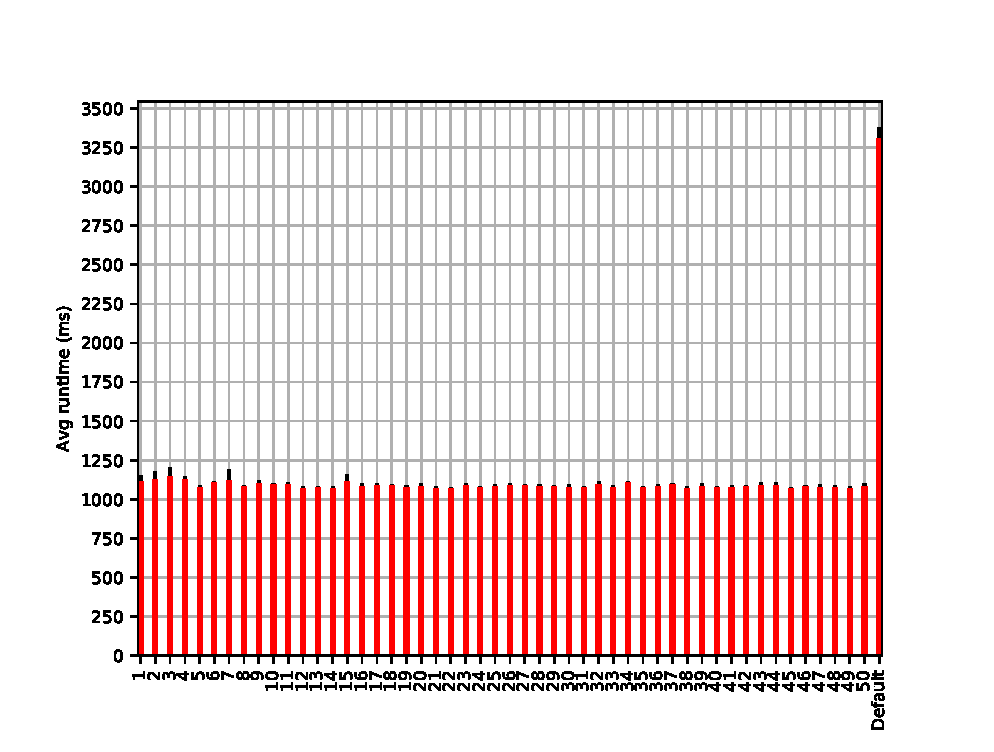
\includegraphics[scale=0.8]{D:/Studie/Master/ExperimentationProject/Results/reorder_comp0_version1.eps}
\caption{Runtimes per target, compiler=0, version=1}
\end{figure}

\begin{figure}[h!]
\centering
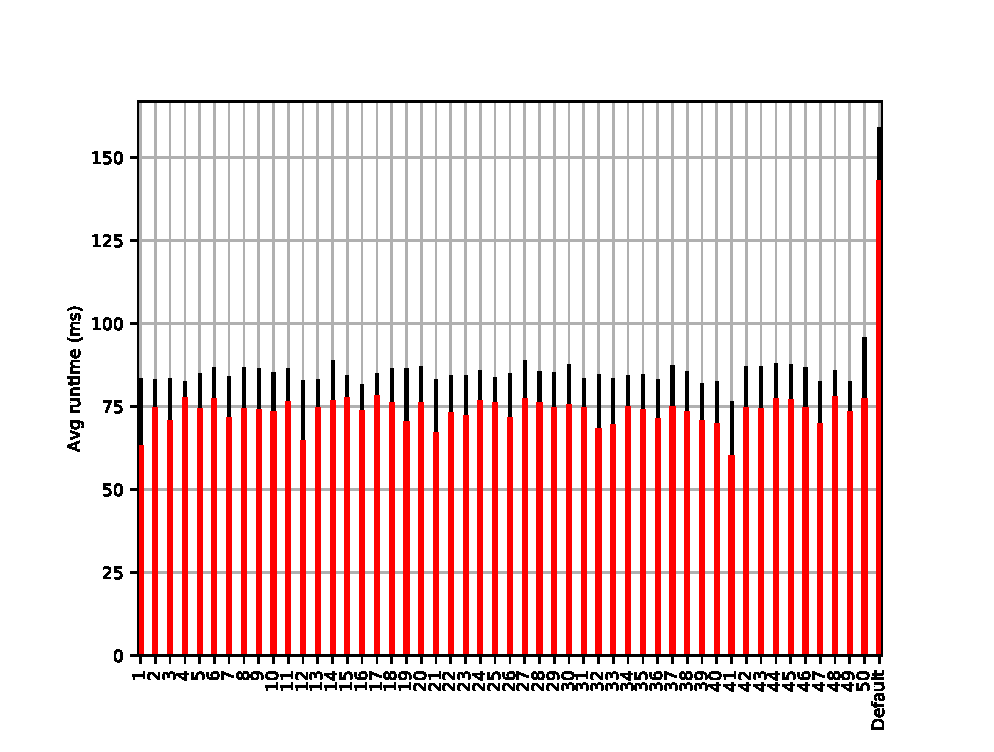
\includegraphics[scale=0.8]{D:/Studie/Master/ExperimentationProject/Results/reorder_comp3_version1.eps}
\caption{Runtimes per target, compiler=3, version=1}
\end{figure}

\begin{figure}[h!]
\centering
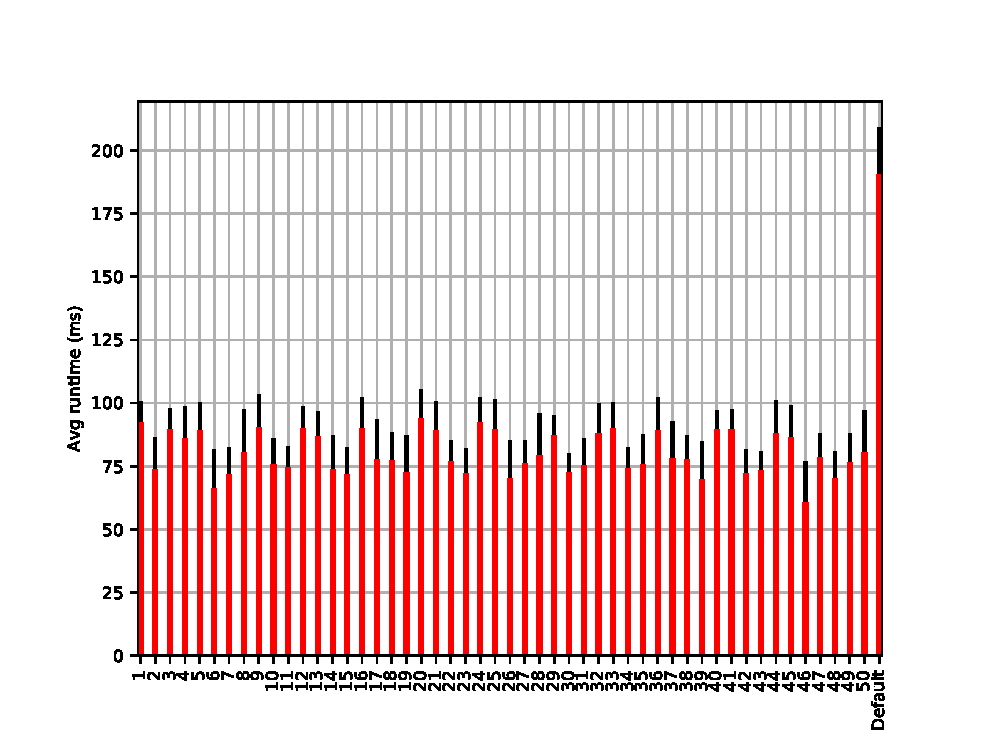
\includegraphics[scale=0.8]{D:/Studie/Master/ExperimentationProject/Results/reorder_comp3_version2.eps}
\caption{Runtimes per target, compiler=3, version=2}
\end{figure}

\begin{figure}[h!]
\centering
\caption{ -corrupt- Runtimes per target, compiler=3, version=3}
\end{figure}

\end{document}

